\section{Supplementary: Experimental Detail and Cost-Survey Forensics}
\label{sec:suppl:experiments}

This supplementary atom carries the operational detail removed from \S\ref{sec:experiments} for the CVPR main paper: the cost-survey micro-grid and production sweep numerics, the $\tau_{\max}$ sensitivity sweep, the rescale-vs-trained checkpoint comparison table, the cost-survey companion figures, and the cross-physics convergence trajectories.

\subsection{Pipeline validation}
\label{sec:suppl:exp:pipeline}
The differentiable integrator was re-validated end-to-end at production architecture (8-layer / 256-unit MLP, $L = 10$ Fourier features, 494{,}084 parameters plus the scalar $\log\tau_{\text{amp}}$), and the cloud loop --- AWS SageMaker \texttt{ml.g5.xlarge} (A10G, 24 GB) with S3 checkpoint sync --- was cleared at the full production schedule on Physics 1, $n_{\text{rays}} = 64$. Peak VRAM at the smallest tier is $\TonePeakVRAM$ GB, the anchor from which the per-tier microbatch table (suppl.\ Tab.~\ref{tab:per-tier-vram}) is derived under the [D-23] linear-VRAM model.

\subsection{Stage 2b: Cost-survey micro-grid (16-cell cross-physics validation)}
\label{sec:suppl:exp:microgrid}
The cost-survey window opens with a 16-cell micro-grid (4 physics $\times$ 4 tiers) at \texttt{max\_steps=200} per cell, dispatched after the [D-24] loss-form revision and the loader saturated-absorber mask landed. Each cell runs the full per-tier microbatch and gradient-accumulation configuration but with a reduced step count, so the matrix is cheap calibration evidence rather than a science-binding result; under [D-23] the cost-survey runs do not gate the [D-13] Stage 2b scientific criteria.

\textbf{Headline outcome.} 16/16 cells PASS the [D-19] descent gate (descent ratio $\leq 0.85$ from step 10 to step 200; observed range $[\MicrogridDescentRangeLo, \MicrogridDescentRangeHi]$, i.e., 25--44\% reduction). Cross-physics \texttt{mean\_flux\_pred} at step 200 spans $\MicrogridMeanFLo$--$\MicrogridMeanFHi$, a spread of \textbf{\MicrogridMeanFSpreadAbs} ($\MicrogridMeanFSpread$) within the 5\% inter-cell consistency bar; the cells were trained against the broken anchor $0.877$ retracted in [D-34], so the absolute value is not interpreted as agreement with the verified $\langle F\rangle_{\text{obs}}(z=0.3) = \AnchorMeanF \pm \AnchorMeanFsigma$. The cross-physics step-1 \texttt{loss\_data} spread under raw-$\tau$ MSE was $\sim 10^{10} \times$ (P1 $\sim 0.05$, P2 $\sim 5 \times 10^{8}$); under the log1p+cap+mask loss the step-200 spread is $[\MicrogridLossDataStepTwoHundredLo, \MicrogridLossDataStepTwoHundredHi]$, i.e., the cross-physics scale anomaly is closed. \texttt{tau\_amp} drift at step 200 is $\MicrogridTauAmpLo$--$\MicrogridTauAmpHi$ across all 16 cells (small, consistent).

\textbf{Memory linearity.} Peak VRAM by tier is $\TonePeakVRAMcell$ GB (T1, chunk 64), $\TtwoPeakVRAMcell$ GB (T2, chunk 256), $\TthreePeakVRAM$ GB (T3, chunk 256, accum 4), and $\TfourPeakVRAM$ GB (T4, chunk 256, accum 64). The linear-VRAM model $\hat{V}_{\text{peak}} \approx \TonePeakVRAM \cdot \min(n_{\text{rays}}, \mu\text{batch}) / 64$ GB is validated to within $\approx 0.5$ GB across $\text{accum\_steps} \in \{1, 4, 64\}$, retroactively satisfying the measured-VRAM gate for the deferred T4 tier.

\subsection{Stage 2b: Cost-survey production sweep (Tier-2 detail)}
\label{sec:suppl:exp:cost-survey-sweep}
The cost-survey production sweep ran the per-tier schedule across all four feedback variants at Tiers 1--3; Tier 4 is currently blocked on the Wrinkle-1 diagnostic. Per [D-23] the cost-survey runs report per-tier final \texttt{loss\_data}, \texttt{mean\_flux\_pred}, \texttt{tau\_amp}, \texttt{peak\_vram\_gb}, and seconds-per-step; they are calibration evidence for the per-tier training schedule, not the [D-13] scientific gates. Tier-1 throughput converged to $\TonePerStepSec$ s/step across all four physics with \texttt{peak\_vram\_gb} held at the $\TonePeakVRAM$ GB micro-grid anchor; Tier-2 and Tier-3 reach \texttt{peak\_vram\_gb} $= \TtwoPeakVRAM$ and $\TthreePeakVRAMprod$ GB respectively, identical to four decimals across physics within each tier. All 12 banked cells PASS the [D-19] safety rails; full per-cell records are in the LEDGER \S6 cost-survey tables.

Tab.~\ref{tab:batch2-t2-cost-survey} fronts three cross-physics observations: (i) physics-invariant peak VRAM at $\TtwoPeakVRAM$ GB; (ii) cross-physics \texttt{mean\_flux\_pred} spread $\TtwoMeanFSpread$; (iii) \texttt{loss\_data} spread $\TtwoLossDataSpread$ ($0.0024$--$0.0028$) --- all consistent with the [D-24] log1p+cap+mask supervision converging symmetrically across the four feedback variants. The cross-cell \texttt{mean\_flux\_pred} consistency is a within-run inter-cell observation; no comparison to the broken-anchor target $0.877$ is asserted (see the [D-34] retraction in \S\ref{sec:experiments:cost-survey-sweep}). Fig.~\ref{fig:cross-physics-convergence} shows the trajectory.

\begin{figure}[t]
    \centering
    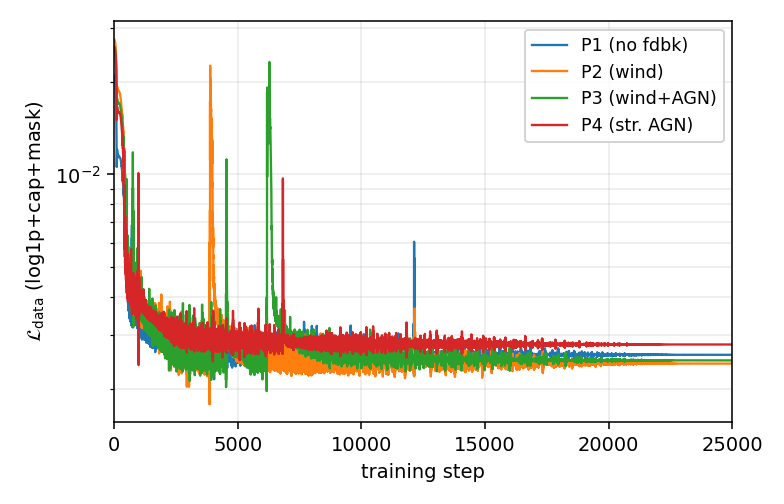
\includegraphics[width=\columnwidth]{figures/cross_physics_convergence.png}
    \caption{Cross-physics convergence under [D-24] log1p+cap+mask supervision, Tier-2 cost-survey ($n_{\text{rays}}=256$, microbatch $1024$, accum $1$, max\_steps $25{,}000$). All four feedback variants converge symmetrically with no divergent trajectory; final $\mathcal{L}_{\text{data}}$ spans $0.00243$--$0.00280$ (a $14.5\%$ relative spread). This closes the cross-physics scale anomaly that raw-$\tau$ MSE exhibited at the same architecture: under the superseded loss form, the step-1 cross-physics $\mathcal{L}_{\text{data}}$ spread was $\sim 10^{10}\times$ (P1 $\sim 0.05$ vs.\ P2 $\sim 5\times 10^{8}$); under [D-24] the four trajectories overlap to within a factor of $1.4$ from step 1. Source data: Sherwood Tier-2 cost-survey runs on Juno HPC.}
    \label{fig:cross-physics-convergence}
\end{figure}

\begin{table}[t]
    \centering
    \renewcommand{\arraystretch}{1.15}
    \setlength{\tabcolsep}{4pt}
    \begin{tabular}{l|cccc}
    Physics & \texttt{loss\_data} & \texttt{mean\_F} & \texttt{tau\_amp} & \texttt{vram\_gb} \\
    \hline
    P1 & \TtwoLossDataPone & \TtwoMeanFPone & \TtwoTauAmpPone & \TtwoPeakVRAM \\
    P2 & \TtwoLossDataPtwo & \TtwoMeanFPtwo & \TtwoTauAmpPtwo & \TtwoPeakVRAM \\
    P3 & \TtwoLossDataPthree & \TtwoMeanFPthree & \TtwoTauAmpPthree & \TtwoPeakVRAM \\
    P4 & \TtwoLossDataPfour & \TtwoMeanFPfour & \TtwoTauAmpPfour & \TtwoPeakVRAM \\
    \end{tabular}
    \caption{Tier-2 cost-survey final-state metrics, one row per physics. Configuration: $n_{\text{rays}}=256$, \texttt{microbatch}$=1024$, \texttt{accum\_steps}$=1$, effective \texttt{chunk\_size}$=256$, \texttt{max\_steps}$=25{,}000$. All four cells PASS the [D-19] safety rails; full run records are in the LEDGER \S6 Tier-2 table. \texttt{peak\_vram\_gb} is identical to four decimals across the four cells (physics-invariant), confirming the [D-23] linear-VRAM model. \emph{Note:} training used $\langle F\rangle_{\text{obs}}=0.877$ at $z=0.3$, retracted in [D-34] (verified value $\AnchorMeanF\pm \AnchorMeanFsigma$, \cite{kirkman2007}). \texttt{mean\_flux\_pred} and $\tau_{\text{amp}}$ absolute values are accordingly uninterpretable; inter-cell consistency and the [D-13] structure gates are anchor-invariant.}
    \label{tab:batch2-t2-cost-survey}
\end{table}

\subsection{$\tau_{\max}$ sensitivity gate}
\label{sec:suppl:exp:tau-max-sensitivity}
Three paired P1-T1 cells at the production schedule, swapping only $\tau_{\max} \in \{5, 10, 20\}$, evaluated under the [D-13] inertial range $k_\parallel \in [10^{\PFkLoExp}, 10^{\PFkHiExp}]$ s/km. The gate criterion is $\max(|\Delta P_F/P_F|) \leq \TauMaxSensGate$ between the $\tau_{\max} = 10$ baseline and each of $\{\tau_{\max} = 5, \tau_{\max} = 20\}$. Observed: $\TauMaxSensLoPercent$ ($\tau_{\max} = 5$) and $\TauMaxSensHiPercent$ ($\tau_{\max} = 20$), i.e., $\sim \TauMaxSensFactorUnderLo\text{--}\TauMaxSensFactorUnderHi\times$ under the $\TauMaxSensGate$ bar. \texttt{mean\_flux\_pred} was identical across all three runs ($\TauMaxSensMeanF$). The gate passed and $\tau_{\max} = 10$ is locked. See Fig.~\ref{fig:tau-max-sensitivity}.

\begin{figure}[t]
    \centering
    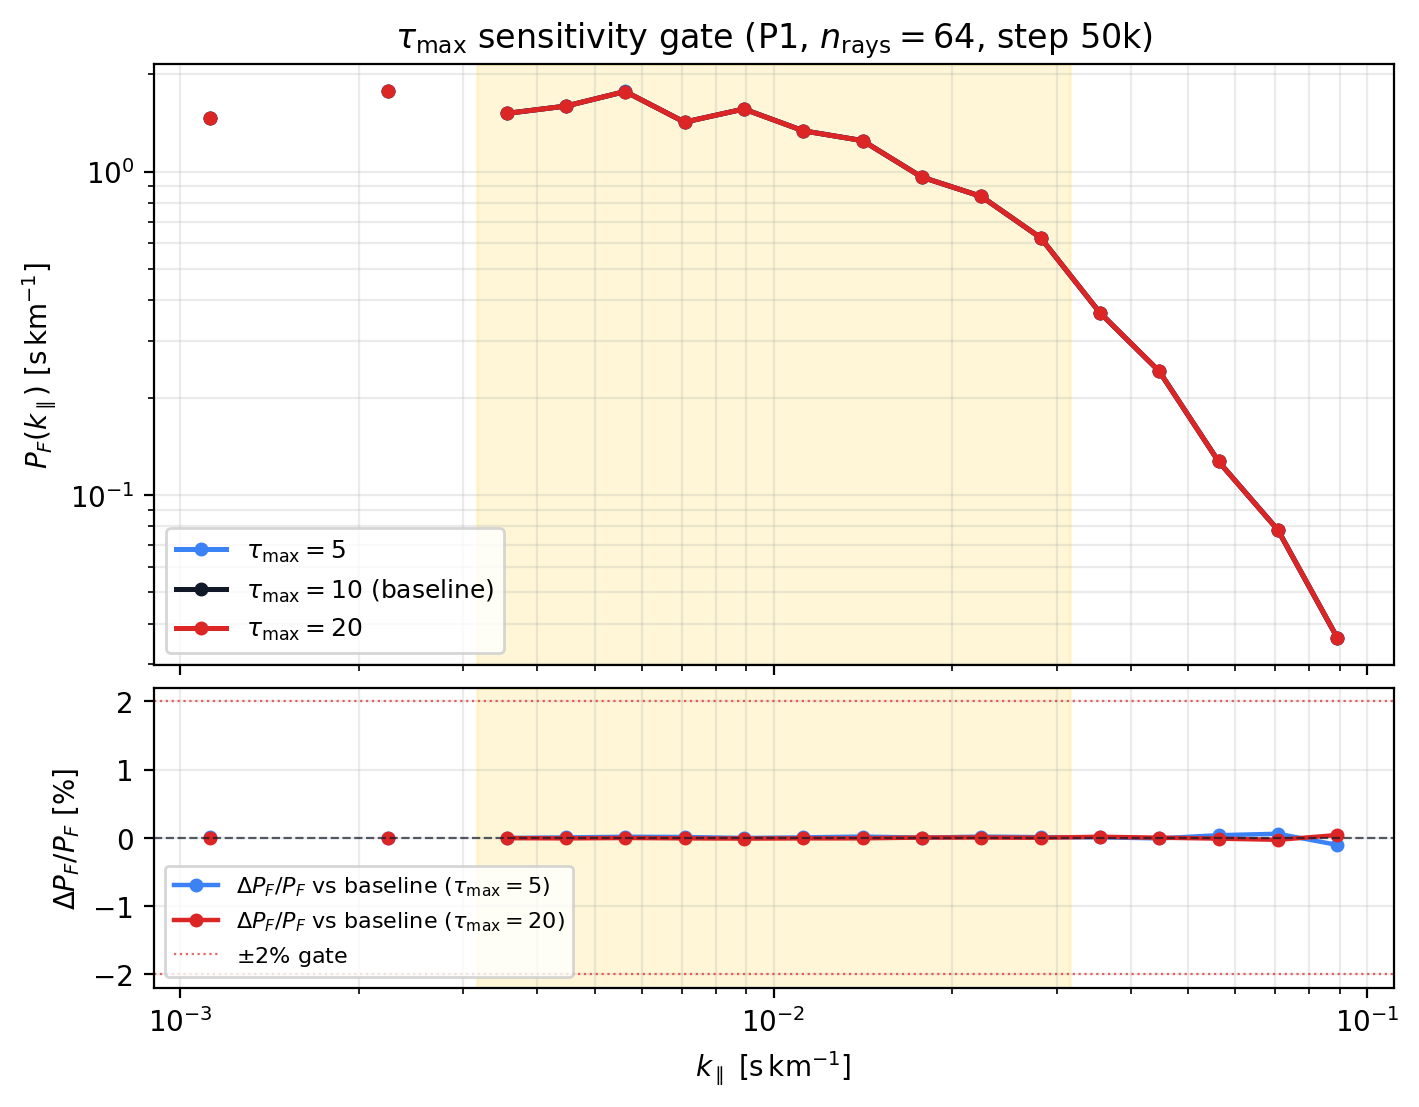
\includegraphics[width=\columnwidth]{figures/tau_max_sensitivity.png}
    \caption{$\tau_{\max}$ sensitivity gate, P1-T1 ($n_{\text{rays}} = 64$, step 50{,}000). Top: 1D flux power spectrum $P_F(k_\parallel)$ for the three caps. Bottom: fractional residual $\Delta P_F / P_F$ vs.\ the $\tau_{\max} = 10$ baseline. Shaded band marks the [D-13] inertial range $k_\parallel \in [10^{\PFkLoExp}, 10^{\PFkHiExp}]$ s/km; dotted lines mark the $\pm \TauMaxSensGate$ gate. Observed maxima ($\TauMaxSensLoPercent$ at $\tau_{\max} = 5$; $\TauMaxSensHiPercent$ at $\tau_{\max} = 20$) clear the gate by $\sim \TauMaxSensFactorUnderLo\text{--}\TauMaxSensFactorUnderHi\times$.}
    \label{fig:tau-max-sensitivity}
\end{figure}

\begin{table}[t]
    \centering
    \renewcommand{\arraystretch}{1.15}
    \begin{tabular}{c|cc|c}
    $\tau_{\max}$ & \texttt{mean\_F} & \texttt{tau\_amp} & $\max(|\Delta P_F/P_F|)$ vs.\ $\tau_{\max}=10$ \\
    \hline
    5  & \TauMaxSensMeanF & 1.152 & $\TauMaxSensLoPercent$ (PASS) \\
    10 & \TauMaxSensMeanF & 1.224 & (baseline) \\
    20 & \TauMaxSensMeanF & 1.234 & $\TauMaxSensHiPercent$ (PASS) \\
    \end{tabular}
    \caption{$\tau_{\max}$ sensitivity sweep numerics for Fig.~\ref{fig:tau-max-sensitivity}. Three paired P1-T1 cells at the production schedule, swapping only the cap. Gate criterion was $\leq \TauMaxSensGate$; both off-baseline cells passed by $\sim \TauMaxSensFactorUnderLo\text{--}\TauMaxSensFactorUnderHi\times$. \texttt{mean\_flux\_pred} is identical across the three runs; the $\sim 7\%$ \texttt{tau\_amp} spread is the expected response to changing the cap on strong-absorber gradients and is absorbed by the [D-21] mean-flux loss. $\tau_{\max} = 10$ is locked.}
    \label{tab:tau-max-sensitivity}
\end{table}

\subsection{Cost-survey-checkpoint companion figures and rescale-vs-trained comparison}
\label{sec:suppl:exp:cost-survey-fig}
Fig.~\ref{fig:p-flux-fiducial}, Fig.~\ref{fig:flux-pdf-fiducial}, and Fig.~\ref{fig:proxy-xi-1d-sample} were generated against the cost-survey T3 checkpoint, on which the rescale-preview framework was originally read. They are retained as the schedule-A reference for the falsification: the rescaled-preview $P_F$ residual at $P_1$ is $\PFrescaledPercent$ under the current pipeline (Fig.~\ref{fig:p-flux-fiducial}, $\PFcostsurveyPoneRaw$ pre-rescale); the trained-at-target $\texttt{pub-t1}$ $P_F$ residual at the same fiducial cell is $\PFresidPonePercent$ (Tab.~\ref{tab:pub-t1-gates}). All $P_F$ residuals quoted in this paper use the post-fix normalized $\delta_F = F/\langle F\rangle - 1$ convention from \texttt{src/analysis/p\_flux.py}; the [D-35] historical-record value $\PFhistoricalDthirtyfive$ is the pre-fix-convention reading.

\begin{figure}[t]
    \centering
    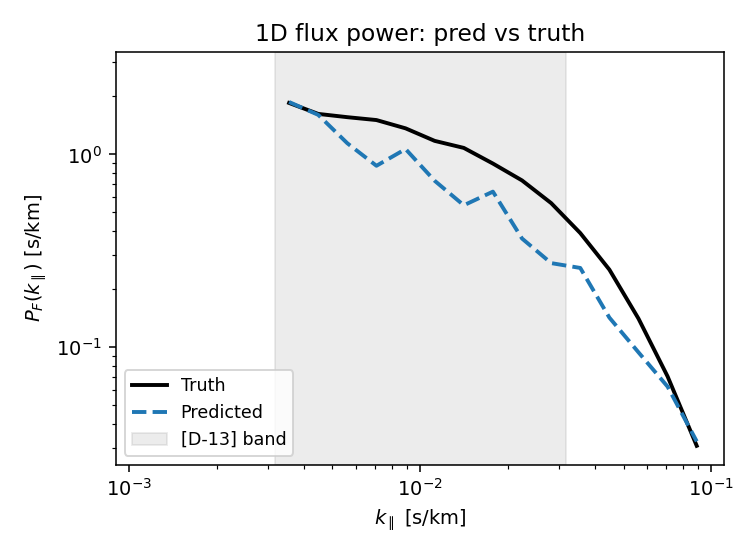
\includegraphics[width=\columnwidth]{figures/d13_pf_fiducial.png}
    \caption{$P_F(k_\parallel)$ reconstruction vs.\ truth at the fiducial point ($P_1$, $z=0.3$, $n_{\text{rays}}=1024$), Tier-3 cost-survey checkpoint (step $10{,}000$). Shaded band marks the [D-13] inertial range $k_\parallel \in [10^{\PFkLoExp}, 10^{\PFkHiExp}]$ s/km. Mean fractional residual in the inertial range: $\mathbf{\PFcostsurveyPoneRaw}$ (gate $<\!\GatePF$, broken-anchor checkpoint; $\PFrescaledPercent$ under the [D-35] uniform rescale to the corrected anchor $\AnchorMeanF$, retracted as preview by [D-39]). The corrected-anchor full-schedule \texttt{pub-t1} measurement at the same fiducial cell gives $|\Delta P_F/P_F|=\PFresidPonePercent$ (Tab.~\ref{tab:pub-t1-gates}): $4\times$ more training did not reduce the residual.}
    \label{fig:p-flux-fiducial}
\end{figure}

\begin{figure}[t]
    \centering
    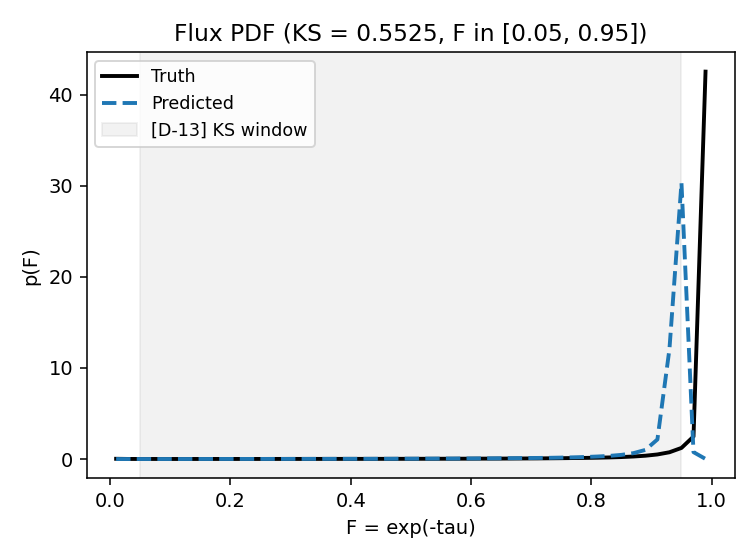
\includegraphics[width=\columnwidth]{figures/d13_flux_pdf_fiducial.png}
    \caption{Flux PDF predicted vs.\ ground-truth, fiducial point, Tier-3 cost-survey. KS distance (cuts $F\in[\PDFwinLo, \PDFwinHi]$): $\mathbf{\KScostsurveyPoneRaw}$ on the broken-anchor checkpoint, $\KScostsurveyPoneRescaled$ after the [D-35] rescale to the corrected anchor (gate $<\!\GateKS$, PASS post-rescale; rescale-as-preview retracted by [D-39]). The corrected-anchor full-schedule \texttt{pub-t1} bundle measures KS$=\KSseedFortyTwoPone$ at $P_1$ and PASSes the gate in $3/4$ cells (Tab.~\ref{tab:pub-t1-gates}); the flux PDF closes while $P_F$ does not.}
    \label{fig:flux-pdf-fiducial}
\end{figure}

\begin{figure}[t]
    \centering
    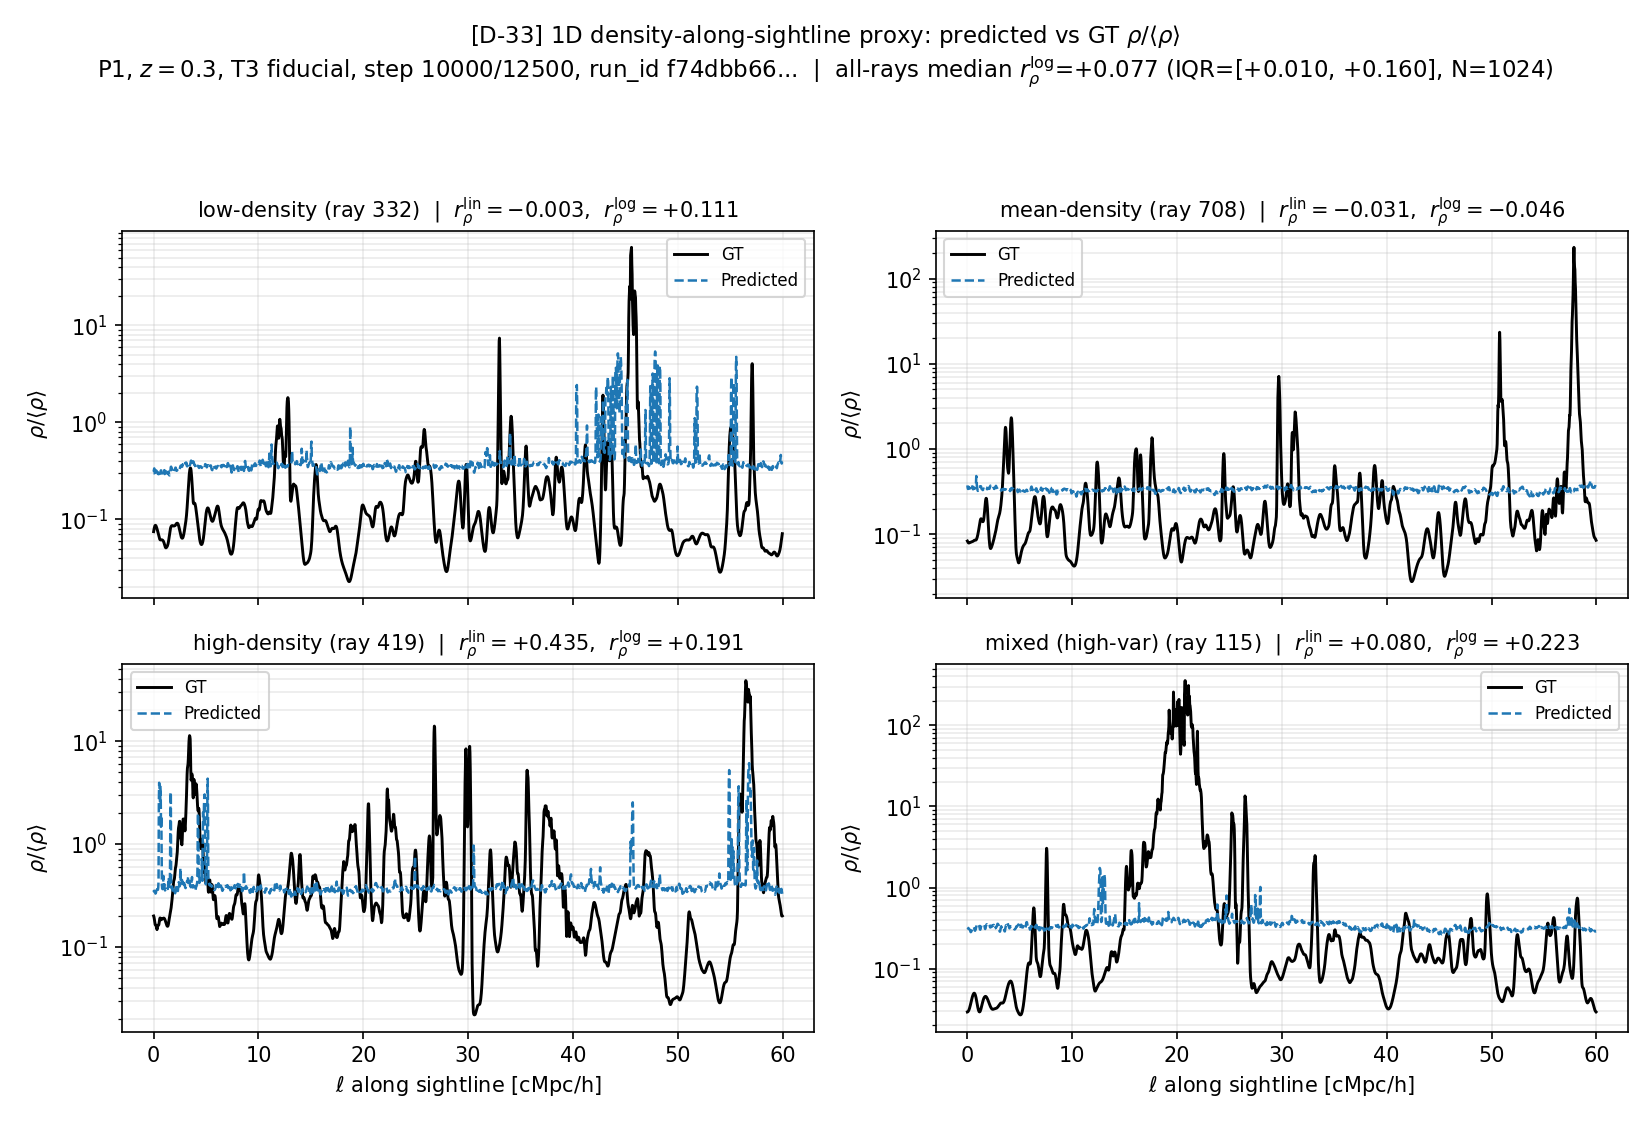
\includegraphics[width=\columnwidth]{figures/proxy_xi_1d_sample.png}
    \caption{\textbf{[D-33] 1D density-along-sightline proxy at T3-$P_1$ fiducial, step $10{,}000/12{,}500$.} Predicted (dashed blue) vs.\ ground-truth (solid black) $\rho/\langle\rho\rangle$ along four representative validation sightlines (low / mean / high density and high-variance), sampled at integrator quadrature points (run\_id \texttt{f74dbb669c\dots}, $P_1$, $z=0.3$, $N=1024$ sightlines). Median per-sightline Pearson correlation on $\log_{10}\rho/\langle\rho\rangle$ is $\mathbf{\rrhoLogProxyPone}$ (IQR $[\rrhoLogProxyIQRLo, \rrhoLogProxyIQRHi]$; 16/84 quantiles $[\rrhoLogProxyQLoSixteen, \rrhoLogProxyQHiEightyfour]$), with $\rrhoLogProxyFracNegative$ of sightlines showing negative correlation --- far below the $\sim \GateXi$ CLAMATO-style reconstruction bar~\cite{lee2015}. The proxy is necessary but not sufficient for the deferred 3D $\xi_{\hat\rho,\rho}$ gate; failing it at this schedule is a strong negative signal under the [D-23] cost-survey framing.}
    \label{fig:proxy-xi-1d-sample}
\end{figure}

\begin{table}[t]
    \centering
    \renewcommand{\arraystretch}{1.15}
    \setlength{\tabcolsep}{3pt}
    \footnotesize
    \begin{tabular}{l|c|c|c|c}
    Gate & Pass cond. & Cost-survey (T3, 10k) & Cost-survey rescaled ($r=\AnchorMeanF/\langle\hat F\rangle$) & \texttt{pub-t1} measured ($P_1$, 50k) \\
    \hline
    $|\Delta P_F/P_F|$ (inertial range) & $< \GatePF$ & $31.03\%$ (FAIL $3.1\times$) & $\PFrescaledPercent$ (FAIL $2.6\times$) & $\mathbf{\PFresidPonePercent}$ (\textbf{FAIL} $\mathbf{\PFfactorOverGateHi\times}$) \\
    KS distance, $F$-PDF & $< \GateKS$ & $\KScostsurveyPoneRaw$ (FAIL $11\times$) & $\mathbf{\KScostsurveyPoneRescaled}$ (PASS) & $\mathbf{\KSseedFortyTwoPone}$ (\textbf{PASS}) \\
    $r_\rho^{\log}$ (1D-proxy [D-33])$^\dagger$ & $> \GateXi$ & $\rrhoLogProxyPone$ (FAIL $\sim \rrhoLogProxyFactorBelowBar\times$) & $\rrhoLogProxyPone$ (anchor-invariant) & (owed: \S\ref{sec:experiments:compute}) \\
    \end{tabular}
    \caption{\textbf{[D-13] structure-gate evaluation at the $P_1$ fiducial point, three checkpoints.} \emph{Superseded by [D-39]; rescaled column retained as upper-bound optimism that the trained \texttt{pub-t1} result falsifies.} Cost-survey column: T3 step $10{,}000/12{,}500$ from run \texttt{f74dbb669c\dots} trained against broken anchor $0.877$. Rescaled column: uniform $\hat{F} \to (\AnchorMeanF/\langle\hat{F}\rangle)\cdot\hat{F}$ applied post-hoc, read by [D-35] as a partial preview of the corrected-anchor publication run. \texttt{pub-t1} measured column: $P_1$ at the corrected-anchor full-schedule run (step $50{,}000$, run \texttt{31acdf9d\dots}). \textbf{Verdict ([D-39]): the rescaled-preview interpretation is falsified.} $P_F$ is the binding gate of any successor run. $^\dagger$1D-along-ray proxy: per-sightline Pearson $r$ on $\log_{10}\rho/\langle\rho\rangle$ at integrator quadrature points; \emph{necessary but not sufficient} for the deferred 3D $\xi_{\hat\rho,\rho}(r)$.}
    \label{tab:d13-gates}
\end{table}

\subsection{$P_F$-overlay falsification figure}
\label{sec:suppl:exp:pf-overlay}
\begin{figure}[t]
    \centering
    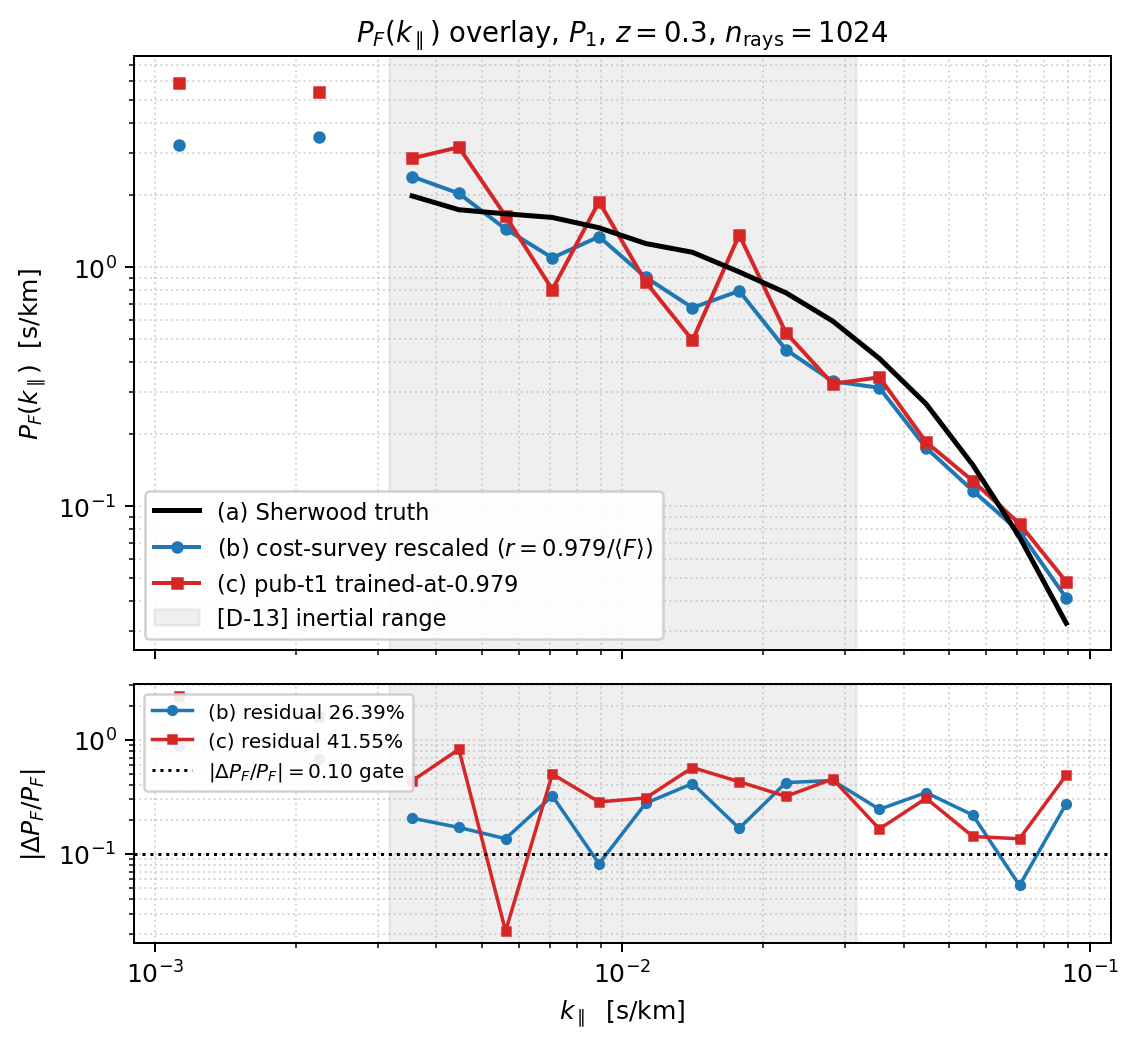
\includegraphics[width=\columnwidth]{figures/pf_overlay_falsification.png}
    \caption{\textbf{$P_F(k_\parallel)$ overlay at $P_1$, $z{=}0.3$, $n_\mathrm{rays}{=}1024$, eval seed $=42$, falsifies the rescale-as-preview interpretation.} Curves: (a) Sherwood ground truth, (b) cost-survey checkpoint after uniform rescale to $\langle F\rangle{=}\AnchorMeanF$ ($|\Delta P_F/P_F|=\PFrescaledPercent$), (c) \texttt{pub-t1} corrected-anchor full-schedule reconstruction ($|\Delta P_F/P_F|=\PFresidPonePercent$). Shaded band: [D-13] inertial range $k_\parallel \in [10^{\PFkLoExp}, 10^{\PFkHiExp}]$ s/km; dotted line: $|\Delta P_F/P_F|{=}\GatePFdec$ gate. $4\times$ more training and the corrected anchor increased the $P_F$ residual by $\Delta=+\PFdriftDeltaPP$ pp.}
    \label{fig:pf-overlay-falsification}
\end{figure}

\subsection{Single-seed seed=42 anchor values (\texttt{pub-t1})}
\label{sec:suppl:exp:pub-t1-anchor}
The single-seed seed=42 anchor row backing the main bootstrap table (main Tab.~\ref{tab:headline-3gate}).

\begin{table}[t]
    \centering
    \renewcommand{\arraystretch}{1.15}
    \setlength{\tabcolsep}{3pt}
    \footnotesize
    \begin{tabular}{l|cccccc}
    Cell & $\langle F_{\text{pred}}\rangle$ & KS ($<\!\GateKS$) & $|\Delta P_F/P_F|$ ($<\!\GatePFdec$) & [D-19] & $\mathcal{L}_{\text{data}}$ (final) & verdict \\
    \hline
    $P_1$ (no fdbk)    & $\meanFseedFortyTwoPone$ & $\KSseedFortyTwoPone$ (PASS) & $\mathbf{\PFresidPone}$ (FAIL $\mathbf{\PFfactorOverGateHi\times}$) & PASS & $\dataMSEPone$ & FAIL on $P_F$ \\
    $P_2$ (wind)       & $\meanFseedFortyTwoPtwo$ & $\mathbf{\KSseedFortyTwoPtwo}$ (FAIL $1.5\times$) & $\mathbf{\PFresidPtwo}$ (FAIL $3.8\times$) & PASS & $\dataMSEPtwo$ & FAIL on $P_F$, KS \\
    $P_3$ (wind+AGN)   & $\meanFseedFortyTwoPthree$ & $\KSseedFortyTwoPthree$ (PASS) & $\mathbf{\PFresidPthree}$ (FAIL $\mathbf{\PFfactorOverGateLo\times}$) & PASS & $\dataMSEPthree$ & FAIL on $P_F$ \\
    $P_4$ (strong AGN) & $\meanFseedFortyTwoPfour$ & $\KSseedFortyTwoPfour$ (PASS) & $\mathbf{\PFresidPfour}$ (FAIL $\mathbf{\PFfactorOverGateLo\times}$) & PASS & $\dataMSEPfour$ & FAIL on $P_F$ \\
    \end{tabular}
    \caption{\textbf{[D-13] structure gates at the seed=42 single-seed anchor, four feedback variants ([D-39]).} Configuration: \texttt{pub-t1}, $n_{\text{rays}}=64$, \texttt{max\_steps}$=50{,}000$, \texttt{microbatch}$=1024$, seed $=0$, $\langle F\rangle_{\text{obs}}=\AnchorMeanF$~\cite{kirkman2007}. MLflow run IDs: \texttt{31acdf9d\dots} ($P_1$), \texttt{f7fafa23\dots} ($P_2$), \texttt{62aeb93a\dots} ($P_3$), \texttt{fc3817b3\dots} ($P_4$); tag \texttt{juno\_batch=pub-t1} on Juno a30. \textbf{Mean-flux PASS $4/4$ (cross-physics spread $\meanFseedFortyTwoSpread$, $<\!1\%$); KS PASS $3/4$; $P_F$ PASS $0/4$, uniformly $\PFfactorOverGateLo\times$--$\PFfactorOverGateHi\times$ over the $\GatePFdec$ gate.} \texttt{peak\_vram}$=\peakVRAMPubtone$ GB; \texttt{tau\_amp} $\in[\tauampPubtoneRangeLo, \tauampPubtoneRangeHi]$; no NaN.}
    \label{tab:pub-t1-gates}
\end{table}

\subsection{Decoupling finding: data-MSE $\perp$ spectroscopic gates}
\label{sec:suppl:exp:decoupling}
The four \texttt{pub-t1} cells reached final $\log(1+\tau)$-MSE values of $\{\dataMSEPone, \dataMSEPtwo, \dataMSEPthree, \dataMSEPfour\}$ at $P_1$/$P_2$/$P_3$/$P_4$ --- spanning four orders of magnitude --- without correspondingly resolving the $P_F$ inertial-range residual (uniform $0.36$--$0.42$ across the same four cells). Log-space MSE on $\tau$ is not a sufficient proxy for the [D-13] spectroscopic gates: the supervision signal saturates well before the second-order flux-power statistic does. We record this as a methodology finding independent of any single physics cell.

\subsection{Saturation-band concentration ratio $R$, per-cell breakdown}
\label{sec:suppl:exp:tau-binned-R-table}
\begin{table}[t]
    \centering
    \renewcommand{\arraystretch}{1.15}
    \setlength{\tabcolsep}{6pt}
    \begin{tabular}{l|cc|c}
    Cell & $|\Delta P_F/P_F|$ & $R$ (sat band) & call \\
    \hline
    $P_1$ (no fdbk)     & \PFresidPone & \RsatPone & PASS positive-ID \\
    $P_2$ (wind)        & \PFresidPtwo & \RsatPtwo & PASS positive-ID \\
    $P_3$ (wind+AGN)    & \PFresidPthree & \RsatPthree & PASS positive-ID \\
    $P_4$ (strong AGN)  & \PFresidPfour & \RsatPfour & PASS positive-ID \\
    \end{tabular}
    \caption{\textbf{Saturation-band concentration ratio $R$ over the four \texttt{pub-t1} cells.} $R = (\text{residual-mass share})/(\text{pixel-mass share})$ in the saturation band $F \in [\SatBandLo, \SatBandHi]$ (bin 7 of the [D-24] partition). Positive-ID floor: $R \geq \GateRsatFloor$. Verdict: \textbf{PASS in 4/4 cells} by $>\!\RsatFactorOverFloor\times$; cross-physics range $\RsatRangeLo$--$\RsatRangeHi$ ($\sim\!\RsatSpreadRelative$ relative spread); $P_4$ (strongest feedback) shows the largest $R$. Per-cell breakdown of the headline number cited in the abstract; the load-bearing visual is Fig.~\ref{fig:all-residual}. Configuration: corrected-anchor full schedule (step $50{,}000$, seed $=42$, $n_{\text{rays}}=1024$, $\langle F\rangle_{\text{obs}}=\AnchorMeanF$).}
    \label{tab:tau-binned-R}
\end{table}

\begin{figure*}[t]
    \centering
    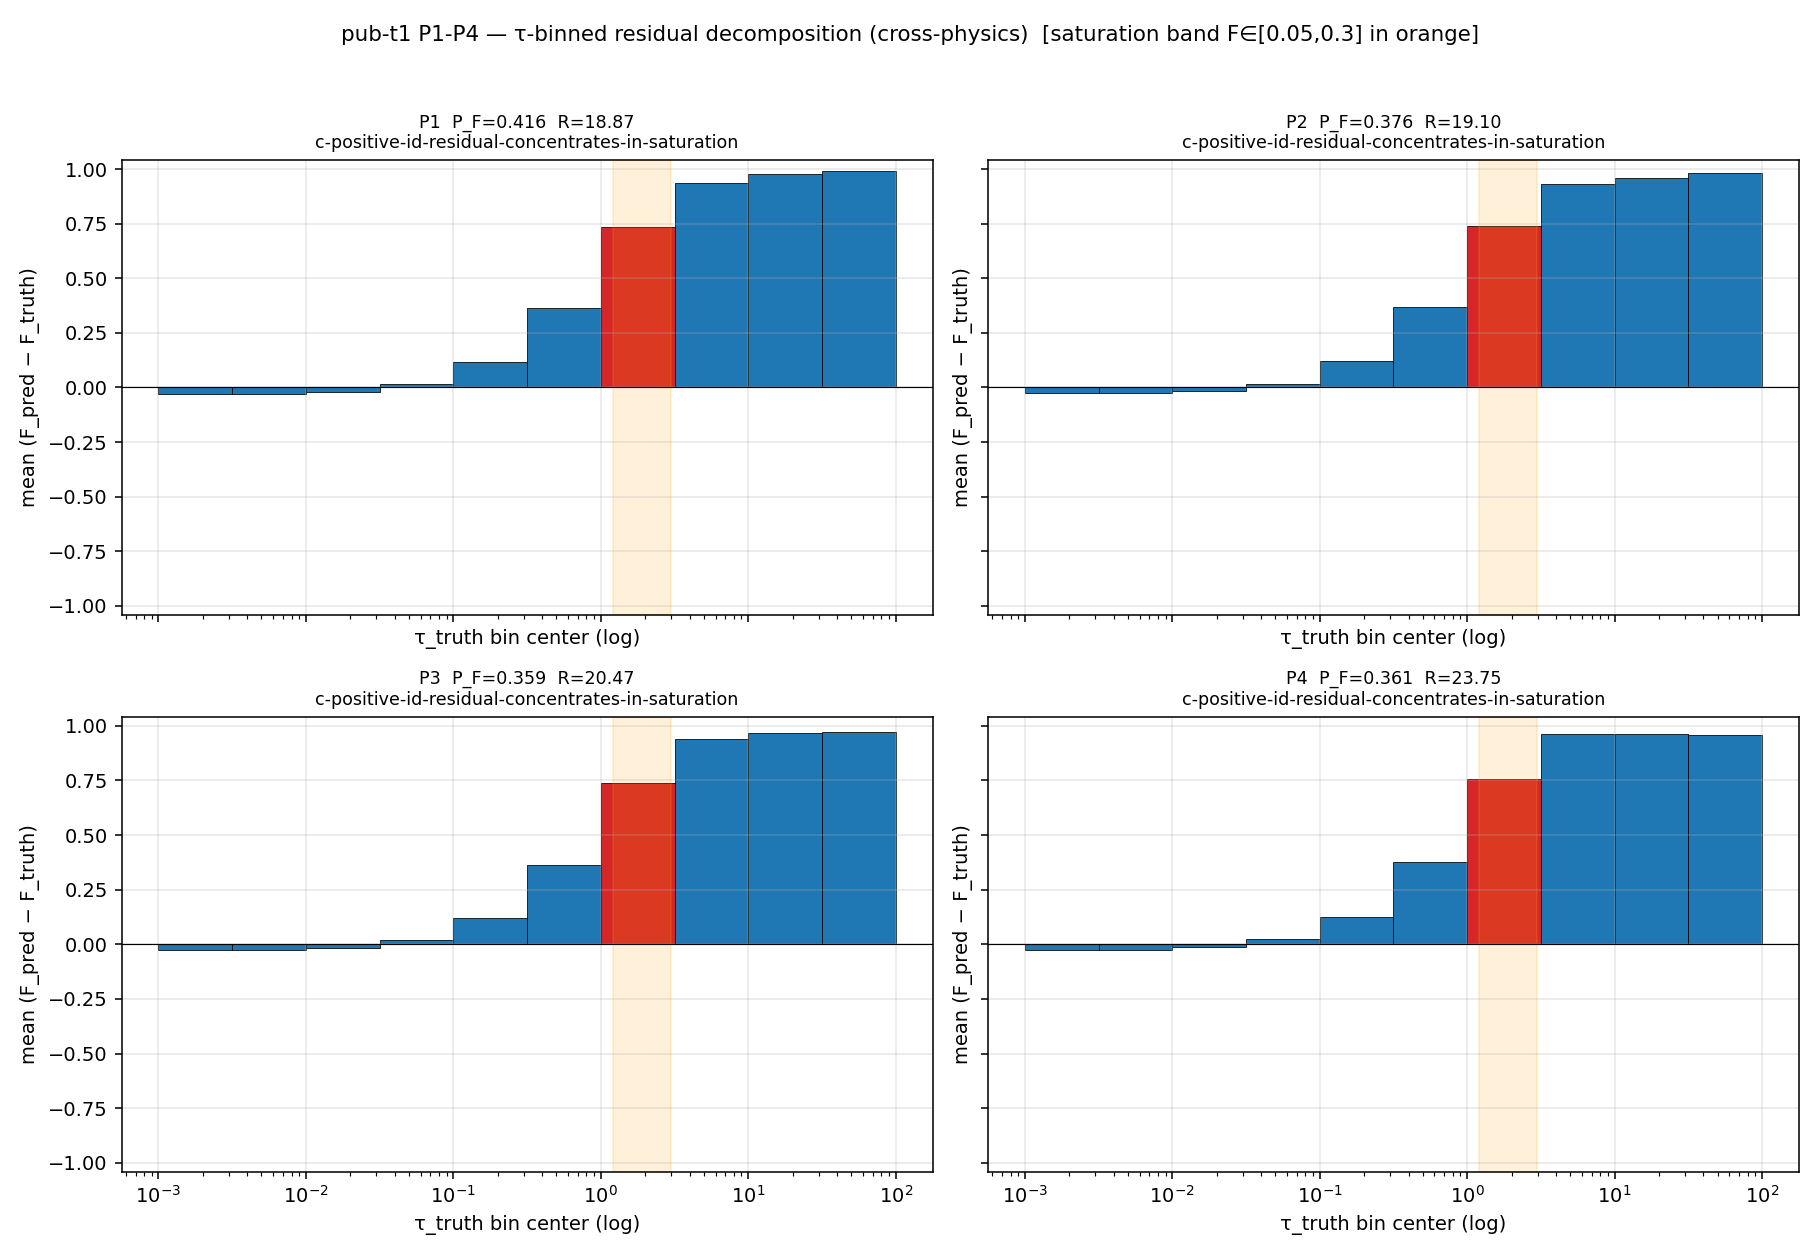
\includegraphics[width=\textwidth]{figures/tau_binned_all_residual.png}
    \caption{\textbf{$\tau$-binned residual decomposition across all four Sherwood feedback variants, positively identifies saturation-regime under-fitting cross-physics.} Configuration: \texttt{pub-t1} corrected-anchor full-schedule checkpoints at step $50{,}000$, seed $=42$, $n_{\text{rays}}=1024$, $\langle F\rangle_{\text{obs}}=\AnchorMeanF$~\cite{kirkman2007}. Each panel: per-bin residual mass $\sum|\Delta F|$ (bars) vs.\ pixel-mass share (dashed) across the seven $F$-bins of the [D-24] saturated-absorber partition; shaded region marks the saturation band $F \in [\SatBandLo, \SatBandHi]$. Saturation-band concentration ratios are $R = \RsatPone$ ($P_1$), $\RsatPtwo$ ($P_2$), $\RsatPthree$ ($P_3$), $\RsatPfour$ ($P_4$); positive-ID floor $R \geq \GateRsatFloor$; observed range $\mathbf{\RsatRangeLo}$--$\mathbf{\RsatRangeHi}$ (cross-physics spread $\sim\!\RsatSpreadRelative$ relative), \textbf{PASS in 4/4 cells} by $>\!\RsatFactorOverFloor\times$ the floor. Linear regime $F > 0.9$ contributes $|\langle \Delta F\rangle| \leq \RsatLinearBandResidual$ per cell; in-band Pearson $r_{\text{pearson}}(\tau) = \RsatPearsonTauPone$ at $P_1$ rules out a uniform $\tau$ rescaling. Verdict: \emph{positively identified residually-supported mechanism cross-physics}; counterfactual closure deferred (main paper \S4). Source: \texttt{scripts/tau\_binned\_residual.py --cell all}. Moved here from the 8-pp main per the CVPR 6-pp cut (2026-05-11).}
    \label{fig:all-residual}
\end{figure*}

\subsection{Sightline-density $\times$ physics-feedback degradation matrix}
\label{sec:suppl:exp:ablation-matrix}
\begin{table}[t]
    \centering
    \renewcommand{\arraystretch}{1.15}
    \setlength{\tabcolsep}{4pt}
    \begin{tabular}{l|cccc}
    Physics & T1 ($n_{\text{rays}}=64$) & T2 ($256$) & T3 ($1024$) & T4 ($16{,}384$) \\
    \hline
    P1 (no fdbk)       & 0.9282 / 1.224 & \TtwoMeanFPone / \TtwoTauAmpPone & 0.9283 / 0.9947 & --- \\
    P2 (wind)          & 0.9247 / 2.315 & \TtwoMeanFPtwo / \TtwoTauAmpPtwo & 0.9269 / 1.0215 & --- \\
    P3 (wind+AGN)      & 0.9275 / 2.038 & \TtwoMeanFPthree / \TtwoTauAmpPthree & 0.9271 / 1.0255 & --- \\
    P4 (strong AGN)    & 0.9308 / 1.955 & \TtwoMeanFPfour / \TtwoTauAmpPfour & 0.9307 / 1.0217 & --- \\
    \end{tabular}
    \caption{Sightline-density $\times$ physics-feedback degradation matrix. Each cell reports \texttt{mean\_flux\_pred} / \texttt{tau\_amp} at the production schedule (50{,}000 steps for T1; 25{,}000 steps for T2; 12{,}500 steps for T3 per [D-23]); all twelve cells PASS the [D-19] safety rails. Source: LEDGER \S6 cost-survey tables under the [D-24] log1p+cap+mask loss. Cross-physics inter-cell mean-flux spreads tighten with rising sightline density: $0.66\%$ (T1) $\to$ $\TtwoMeanFSpread$ (T2) $\to$ $0.41\%$ (T3). Tier 4 is currently blocked on the Wrinkle-1 diagnostic ([D-39]). \emph{Note:} training used $\langle F\rangle_{\text{obs}}=0.877$ at $z=0.3$, retracted in [D-34]. \texttt{mean\_flux\_pred} and $\tau_{\text{amp}}$ absolute values are accordingly uninterpretable; inter-cell consistency and the [D-13] structure gates are anchor-invariant.}
    \label{tab:ablation-matrix}
\end{table}

\subsection{Supplementary view at fiducial $P_1$ ($\tau$-binned single-cell decomposition)}
\label{sec:suppl:exp:tau-binned-p1}
The $P_1$-only single-panel decomposition (\texttt{p1\_residual.png}) is the higher-resolution companion to Fig.~\ref{fig:all-residual}. The single-cell view exposes per-bin $\langle \Delta \tau\rangle$ and $r_{\text{pearson}}(\tau)$ numerics that the four-panel composite compresses for shared-axis comparability; both figures share the same artifact pipeline and pass the same $R \geq \GateRsatFloor$ gate at $P_1$ ($R = \RsatPone$). Track-wide $R$-uniformity is the headline; the $P_1$ companion is detail.

\subsection{Substrate-scale extension probe at $48^3$}
\label{sec:suppl:exp:substrate-probe-cprime}
The first realized substrate-scale follow-on to the $\SubstrateProbeCropSize^3$ substrate-discriminability probe (\S\ref{sec:experiments:substrate-probe} in the main paper) re-runs the 4-class Sherwood feedback discrimination problem on truth-$\rho$ crops of edge $\SubstrateProbeCpCropSize^3$ voxels. The simulation pitch is held fixed at $n_{\text{grid}}=768$ (per-voxel comoving edge $\SubstrateProbeCpVoxelKpc$~kpc/h, identical to the $\SubstrateProbeCropSize^3$ probe), so only the crop dimension changes; the comparison is a substrate-extent contrast at fixed resolution rather than a resolution contrast~\cite{touvron2019fixres}. The $\SubstrateProbeCpCropSize^3$ cube subtends $\SubstrateProbeCpBoxMpc~h^{-1}$ Mpc on a side, against $\SubstrateProbeBoxMpc~h^{-1}$ Mpc for the $\SubstrateProbeCropSize^3$ baseline. Architecture and readout are unchanged from the $\SubstrateProbeCropSize^3$ probe: a 3D ResNet-18 with halved channel widths ($\SubstrateProbeCpResnetParams$ parameters, \texttt{AdaptiveAvgPool3d(1)} global-average-pool readout), and the test region is drawn from the same axis-0 70/15/15 held-out spatial split.

\paragraph{Five-seed protocol and self-anchored reference.}
The protocol fixes seed sensitivity as a first-class quantity. Five seeds $\{42, 142, 242, 342, 442\}$ are drawn under pre-committed branch routing; each seed produces an independent classifier whose accuracy on $\SubstrateProbeCpNcrops$ test crops contributes one per-crop indicator stream, giving $\SubstrateProbeCpNcropsTotal$ per-crop indicators in total. The aggregation metric is the AD-5 margin between the 3D ResNet truth-discriminator and a moment-only MVSK 4-scalar baseline trained on $\{\text{mean}, \text{variance}, \text{skewness}, \text{kurtosis}\}$ of the same crop --- the same baseline class used in the $\SubstrateProbeCropSize^3$ probe but evaluated at $\SubstrateProbeCpCropSize^3$ crops. The reference at $\SubstrateProbeCpRefPP$~pp is a \emph{self-anchored project-side reference} carried over from the $\SubstrateProbeCropSize^3$ probe design, \emph{not} a published external threshold; it is the bar against which the probe's own pre-committed pass/fail call was made. Both the within-seed paired-classifier correlation $\rho_{\text{emp}}=\SubstrateProbeCpRhoEmp$ (mean across the five seeds) and the between-seed correlation of per-crop ResNet correctness $\rho_{\text{seed,emp}}=\SubstrateProbeCpRhoSeedEmp$ (over the $10$ seed-pairs) are reported as part of the diagnostic stack.

\paragraph{Headline numerics.}
The 3D ResNet attains $5$-seed mean accuracy $\SubstrateProbeCpResnetAcc \pm \SubstrateProbeCpResnetSigma$ (sample standard deviation, $n=5$, $\mathrm{ddof}=1$). The MVSK 4-scalar baseline on the same $\SubstrateProbeCpCropSize^3$ crops attains $\SubstrateProbeCpMvskAcc \pm \SubstrateProbeCpMvskSigma$. The MVSK baseline re-evaluated at $\SubstrateProbeCropSize^3$ crops \emph{inside the same pipeline} (the nested A4 baseline of design v4 §B3/B4) attains $\SubstrateProbeCpMvskAt32cube$ at $5$-seed mean. The AD-5 margin between the ResNet and the MVSK baseline at $\SubstrateProbeCpCropSize^3$ is $\SubstrateProbeCpMarginPP$~pp (point estimate). A $95\%$ bootstrap CI by resampling the $5$ seeds with replacement ($B=\SubstrateProbeCpBootB$, RNG seed $\SubstrateProbeCpBootRng$) gives $[\SubstrateProbeCpCIlow, \SubstrateProbeCpCIhigh]$~pp~\cite{politis_romano1994}; all $5/5$ seeds individually clear the $\SubstrateProbeCpRefPP$~pp self-anchored reference, with the closest-to-bar seed (seed $242$) at $\SubstrateProbeCpMarginSeedTwofortytwo$~pp ($\SubstrateProbeCpClosestSeedFactor\times$ the reference).

\paragraph{Nesting disclosure.}
The MVSK 4-scalar baseline that the AD-5 margin is measured against is itself nested inside the same self-anchored framework that the $\SubstrateProbeCropSize^3$ probe was evaluated against. That is, the reference at $\SubstrateProbeCpRefPP$~pp is the gap a 3D ResNet must clear over an MVSK 4-scalar to be read as carrying signal beyond the moment subspace, where ``signal'' and ``moment subspace'' are both fixed at project-side design time and not against any published external benchmark. We name the nesting explicitly so the substrate-axis reading is not overdrawn into an external claim it does not support: the $\SubstrateProbeCpCropSize^3$ result is a within-framework margin, not a calibration against the literature on 3D-CNN discrimination at this scale.

\paragraph{Seed-variance budget caveat.}
The empirical between-seed standard deviation on the 3D ResNet readout is $\SubstrateProbeCpResnetSigma$, against a pre-committed design budget of $\SubstrateProbeCpSeedBudget$ --- a factor of $\SubstrateProbeCpSeedFactor$ over the budget. The MVSK baseline's between-seed standard deviation is $\SubstrateProbeCpMvskSigma$, within the same budget. The under-estimate on the ResNet side is in the conservative direction relative to the verdict: the effect size at $\SubstrateProbeCpCropSize^3$ is large enough that the AD-5 margin clears the $\SubstrateProbeCpRefPP$~pp reference at all five seeds and the $95\%$ CI lower bound at $\SubstrateProbeCpCIlow$~pp is still $\sim\!1.9\times$ the reference, so the verdict does not flip when the seed variance is read at its empirical value rather than at the design budget. We disclose this anyway, because it confirms the directional risk on discriminative-classifier seed sensitivity that D'Amour et al.~\cite{damour2020underspecification} document as the systematic mode under which this kind of probe is expected to mis-state confidence; an escalation of the protocol (e.g., a tighter seed-variance budget at the $\SubstrateProbeCpSeedFactor\times$ empirical value, or a larger seed schedule) is the obvious follow-on if the substrate-axis reading is taken further.

\paragraph{Single-pair substrate-scale contrast.}
The $(\SubstrateProbeCropSize^3, \SubstrateProbeCpCropSize^3)$ pair, at fixed simulation pitch, is a single-pair contrast. The reading is that at the $\SubstrateProbeCropSize^3$ substrate the 4-class Sherwood feedback signature collapses to within seed noise of the MVSK 4-scalar baseline ($\SubstrateProbeMarginPP$~pp gap against a $\SubstrateProbeADfiveBarPP$~pp reference); at the $\SubstrateProbeCpCropSize^3$ substrate the same problem carries a $\SubstrateProbeCpMarginPP$~pp gap against the same reference. Both readings are complementary records of what the substrate at each configuration affords; the $\SubstrateProbeCpCropSize^3$ reading is \emph{not} a generalization of the $\SubstrateProbeCropSize^3$ reading, and no curve-shape inference is admissible from two points. A multi-point scoping curve, sampling additional substrate edges (e.g., $96^3$ and beyond) at the same fixed pitch, is the natural next step before any verb stronger than ``contrast at $(\SubstrateProbeCropSize^3, \SubstrateProbeCpCropSize^3)$'' can be supported; the present compute budget allowed only this pair. Compute provenance: Juno H100 g-06-01, wallclock $\SubstrateProbeCpWallclock$~min, run \texttt{\SubstrateProbeCpRunId}, Juno job $\SubstrateProbeCpJunoJob$, headline artifact \texttt{cloud\_runs/\SubstrateProbeCpRunTag/eval/headline.json}.

\begin{table}[t]
    \centering
    \renewcommand{\arraystretch}{1.15}
    \setlength{\tabcolsep}{4pt}
    \footnotesize
    \begin{tabular}{l|c|c|c|c}
    Seed & ResNet acc.\ & MVSK acc.\ ($48^3$) & MVSK acc.\ ($32^3$, nested) & AD-5 margin (pp) \\
    \hline
    $42$  & $0.6283$ & $0.3808$ & $0.3969$ & $\SubstrateProbeCpMarginSeedFortytwo$ \\
    $142$ & $0.5578$ & $0.2933$ & $0.3116$ & $\SubstrateProbeCpMarginSeedOnefortytwo$ \\
    $242$ & $0.4705$ & $0.3278$ & $0.3630$ & $\SubstrateProbeCpMarginSeedTwofortytwo$ \\
    $342$ & $0.6663$ & $0.3499$ & $0.2788$ & $\SubstrateProbeCpMarginSeedThreefortytwo$ \\
    $442$ & $0.5799$ & $0.3340$ & $0.3499$ & $\SubstrateProbeCpMarginSeedFourfortytwo$ \\
    \hline
    mean  & $\SubstrateProbeCpResnetAcc$ & $\SubstrateProbeCpMvskAcc$ & $\SubstrateProbeCpMvskAt32cube$ & $\SubstrateProbeCpMarginPP$ \\
    std   & $\SubstrateProbeCpResnetSigma$ & $\SubstrateProbeCpMvskSigma$ & --- & --- \\
    \end{tabular}
    \caption{\textbf{Per-seed substrate-extension probe at $\SubstrateProbeCpCropSize^3$, fixed pitch $n_{\text{grid}}=768$.} 5 seeds $\{42, 142, 242, 342, 442\}$, $\SubstrateProbeCpNcrops$ test crops per seed. Columns 2--3: 3D ResNet-18 and MVSK 4-scalar baseline accuracy on the same $\SubstrateProbeCpCropSize^3$ crops. Column 4: MVSK re-evaluated at $\SubstrateProbeCropSize^3$ crops inside the same pipeline (nested A4 baseline). Column 5: AD-5 margin (ResNet $-$ MVSK at $\SubstrateProbeCpCropSize^3$), in percentage points. All $5/5$ seeds clear the project-side self-anchored $\SubstrateProbeCpRefPP$~pp reference; closest-to-reference seed is $242$ at $\SubstrateProbeCpMarginSeedTwofortytwo$~pp ($\SubstrateProbeCpClosestSeedFactor\times$ reference). 5-seed mean AD-5 margin $\SubstrateProbeCpMarginPP$~pp, $95\%$ bootstrap CI $[\SubstrateProbeCpCIlow, \SubstrateProbeCpCIhigh]$~pp ($B=\SubstrateProbeCpBootB$). Empirical between-seed ResNet $\sigma=\SubstrateProbeCpResnetSigma$ is $\SubstrateProbeCpSeedFactor\times$ the pre-committed design budget $\SubstrateProbeCpSeedBudget$ in the conservative direction (verdict not flipped). Source: \texttt{cloud\_runs/\SubstrateProbeCpRunTag/eval/headline.json}.}
    \label{tab:substrate-probe-cprime-per-seed}
\end{table}
